% Contenidos del capítulo.
% Las secciones presentadas son orientativas y no representan
% necesariamente la organización que debe tener este capítulo.
\section{Implementación}
\subsection{Tecnologías y herramientas}

Primeramente, el motor, como ya se ha mencionado, es Unity, pero para el desarrollo de este se empleó más concretamente la versión 2021.3.9f1. En cuanto a los sistemas de interacción, destacamos dos, el XR Interaction Toolkit 2.3.0 para manejo de mandos VR y el XR Hands Package para soporte de hand tracking. Para la gestión de texto, se ha empleado el TextMesh Pro 3.0.6 con soporte Unicode extendido, que ya posee Unity, y fonts adecuadas. El pluguin OpenXR 1.7.0, nos ha servido de backend multiplataforma. Finalmente, y como ya se ha explicado, se a mantenido un control de versiones con  GitHub.


\subsection{Desafíos técnicos específicos}

\subsubsection{Soporte de carácteres complejos}
Uno de los mayores desafíos radicaba en el correcto renderizado de caracteres poco comunes como los del alfabeto cirílico, el griego y el coreano.

\begin{table}[h]
	\centering
	\begin{tabular}{|l|c|c|}
		\hline
		\textbf{Idioma} & \textbf{Caracteres especiales} & \textbf{Soporte} \\ \hline
		Coreano         & 11,172 sílabas                 & 100\%           \\ \hline
		Griego          & 24 letras + 5 acentos          & 100\%           \\ \hline
		Ruso            & 33 letras                      & 100\%           \\ \hline
	\end{tabular}
	\caption{Validación de caracteres especiales}
	\label{tab:caracteres}
\end{table}

Para ello se necesitó crear un Font Asset personalizado, que tardó 1 día y medio en procesarse, con una font que admitiera todos estos caracteres. En este caso en concreto se optó por utilizar la font NotoSansCJK-Regular, que también cuenta con el soporte de otras grafias asiáticas para posibles ampliaciones futuras.

\begin{figure}[H]
	\centering
	
\includegraphics[width=0.6\textwidth]{FontAsset.png}
	\caption{Font Asset personalizado}
	\label{fig:font_asset}
\end{figure}

\subsubsection{silabas del Hangul}

El otro gran desafió se trato de desarrollar un código que admitiera la formación automática de las silabas del alfabeto hangul. Estas sílabas se forman juntando una consonante inicial(hay 19), una vocal intermedia(hay 21) y una posible consonante final(28). La gran ventaja que se encontró es que las sílabas en las tablas unicode se encontraban repartidas en bloques equitativos de combinaciones, por lo que se pudo desarrollar un algoritmo matemático que saca el índice correcto a partir del índice relativo de las letras que lo forman(se empieza por 0). Este algoritmo trata en coger el índice de la consonante inicial, multiplicarlo por 21, debido a las posibles combinaciones con las vocales, a esto sumarle el índice relativo de la vocal; al resultado se le multiplica por 28 por las combinaciones que tienen todas las sílabas anteriores con las consonantes finales; a este resultado hay que sumarle la consonante final y da el índice relativo de la sílaba; a esto solo queda posicionarlo en la tabla unicode añadiéndole el índice real de la primera sílaba,  que es el OxAC00, en exadecimal, o el 44032, en decimal.

\begin{figure}[H]
	\centering
	
\includegraphics[width=1\textwidth]{Algoritmo.png}
	\caption{Fragmento del código con el algoritmo de la formación de sílabas hangul}
	\label{fig:font_asset}
\end{figure}

Para ayudarme a sacar los índices correctos, me creé unas listas que consulto antes de aplicar el algoritmo.

\begin{figure}[H]
	\centering
	
\includegraphics[width=1\textwidth]{ListasHangul.png}
	\caption{Fragmento del código con las listas}
	\label{fig:font_asset}
\end{figure}

\section{Validando el sistema: Mi experiencia práctica}

Cuando llegó el momento de probar todo lo que había construido, me puse manos a la obra con un par de bebidas energéticas (sin azucar) y mucha paciencia. Lo primero que hice fue sentarme frente al visor VR y empezar a teclear como loco. Metí más de 150 caracteres raros a mano, uno tras otro, para ver si salían bien dibujados. Griego, coreano, cirílico... un montón de símbolos que parecían salidos de otro planeta. Recuerdo especialmente el problema con esa letra rusa "yo" (esa que parece una 'e' con sombrerito) - ¡se veía toda aplastada! Pero después de jugar un rato con los ajustes de TextMesh Pro, por fin quedó decente.

Lo del coreano fue otro mundo. Me pasé una tarde entera probando combinaciones de consonantes y vocales como si fuera un juego de Lego lingüístico. "Vamos a ver, si juntamos H + A + N... ¿saldrá 'han'?" Y ahí estaba, la sílaba 10588 en la tabla Unicode, apareciendo como por arte de magia en la pantalla. Fue uno de esos momentos "¡eureka!" que hacen que todo el esfuerzo valga la pena.

\section{Pruebas de rendimiento}

Te soy sincero, me daba un poco de miedo que todo fuera a explotar en plena demostración. Por eso me puse a observar cómo se comportaba el teclado en el mundo real. Durante las pruebas con mis compañeros, vigilaba como un halcón: ¿se atascaba al escribir? ¿Se cerraba de repente? Para mi alivio, aguantó bien el tipo. Eso sí, noté que en sesiones largas la memoria empezaba a respirar con dificultad, como cuando subes una cuesta con la bici cargada.

El gran susto vino con el Font Asset. ¡Catorce horas generando esa cosa! Me fui a dormir dejando el ordenador trabajando y al despertar... seguía ahí, tostándose como un pollo al horno. El resultado fue que la primera vez que abrías la app, tardaba lo suyo en cargar. Solución: ahora arranca antes que nada, mientras muestro ese logo molón que diseñé.

\section{Lo que aprendí en el camino}

Si hay algo que me quedó claro es que lo de las fuentes multilingües es un infierno. Nunca más quiero pasar otro día entero esperando que se genere un Font Asset. La próxima vez, buscaré fuentes prehechas o las partiré en trocitos. Por otro lado, TextMesh Pro fue mi salvación - sin él esto habría sido imposible.

Sobre la VR, descubrí cosas curiosas. La gente necesita un par de minutos para acostumbrarse al teclado flotante - al principio todos movían las manos como espantando moscas. Y las teclas tienen que ser más grandes de lo que crees, porque en el espacio 3D todo se ve más pequeño. Lo más importante: sin vibración en los mandos, tienes que poner buenas señales visuales, si no la gente no sabe si ha pulsado bien.

Al final, lo que más me llevo es que cada problema tenía solución. A veces tardabas en encontrarla, pero siempre aparecía. Como cuando a las 2 de la mañana se me ocurrió lo de precargar la fuente durante el inicio... ¡y funcionó!

\section{Pruebas de usabilidad}

\subsection{Metodología SUS}

Para este estudio, quise aprovechar que estoy cursando el Grado Superior en Desarrollo de Aplicaciones Multiplataforma. Después de hablar con varios profesores y compañeros, conseguí que 11 estudiantes de mi clase -con edades entre 18 y 28 años- probaran el teclado VR. La verdad es que me sorprendió lo dispuestos que estaban a colaborar. Casi ninguno tenía experiencia previa con realidad virtual (solo dos chicos habían usado algo antes), pero todos manejaban bien los ordenadores y teclados normales, claro, siendo estudiantes de informática.

Antes de empezar, fue importante que cada uno firmara el consentimiento informado \ref{fig:Consentimiento Informado}. No quería dejar nada al azar en ese aspecto. Las pruebas fueron individuales, de unos 15 minutos cada una: primero usaban el teclado, luego rellenaban el cuestionario SUS \ref{fig:Custionario SUS}. Ese formulario tiene su truco - las preguntas pares van "al revés", así que hay que estar atento al puntuar.

Cuando vi los resultados (Tabla \ref{tab:sus_scores}), me llevé una grata sorpresa. Las puntuaciones fueron bastante altas en general. El gráfico de barras (Figura \ref{fig:barras}) muestra claramente cómo la mayoría se concentra arriba del todo. De hecho, si nos fijamos en el pastel (Figura \ref{fig:sus_pie}), más del 70\% de mis compañeros dieron al teclado una nota de usabilidad "excelente". ¡Incluso uno llegó a 95 puntos! Solo tres estuvieron en la franja "aceptable" (entre 68 y 84), y ninguno lo consideró "inaceptable".

Eso sí, noté un patrón curioso: los dos compañeros que dieron las notas más bajas (70 y 77.5) fueron precisamente quienes más problemas tuvieron con los idiomas asiáticos. Uno me comentó después: "Lo del coreano se me hizo cuesta arriba". Pero incluso ellos reconocieron que el teclado funcionaba bien en general.

Personalmente, creo que estos números demuestran que el prototipo va por buen camino, especialmente considerando que casi todos eran nuevos en VR. Eso sí, la parte multilingüe necesita más trabajo, como veremos más adelante.

\begin{table}[H]
	\centering
	\caption{Puntuaciones SUS del teclado VR por alumno}
	\label{tab:sus_scores}
	\begin{tabular}{cccccccccccc}
		\toprule
		\textbf{Alumno} & \textbf{P1} & \textbf{P2} & \textbf{P3} & \textbf{P4} & \textbf{P5} & \textbf{P6} & \textbf{P7} & \textbf{P8} & \textbf{P9} & \textbf{P10} & \textbf{SUS} \\
		\midrule
		1  & 5 & 1 & 5 & 1 & 3 & 2 & 5 & 2 & 4 & 1 & 87.5 \\
		2  & 4 & 2 & 4 & 1 & 5 & 3 & 4 & 1 & 5 & 1 & 85.0 \\
		3  & 3 & 1 & 4 & 1 & 4 & 2 & 5 & 1 & 5 & 1 & 87.5 \\
		4  & 5 & 1 & 4 & 1 & 5 & 2 & 4 & 1 & 5 & 1 & 92.5 \\
		5  & 4 & 1 & 5 & 1 & 5 & 1 & 5 & 1 & 3 & 1 & 92.5 \\
		6  & 4 & 1 & 3 & 1 & 4 & 1 & 5 & 2 & 4 & 1 & 85.0 \\
		7  & 4 & 3 & 4 & 2 & 5 & 2 & 4 & 2 & 5 & 2 & 77.5 \\
		8  & 4 & 1 & 5 & 1 & 4 & 1 & 5 & 1 & 5 & 1 & 95.0 \\
		9  & 5 & 1 & 4 & 2 & 5 & 1 & 4 & 1 & 3 & 1 & 87.5 \\
		10 & 3 & 3 & 5 & 4 & 4 & 2 & 4 & 2 & 4 & 1 & 70.0 \\
		11 & 4 & 1 & 5 & 1 & 4 & 1 & 5 & 1 & 4 & 1 & 92.5 \\
		\bottomrule
	\end{tabular}
\end{table}

\begin{figure}[H]
	\centering
	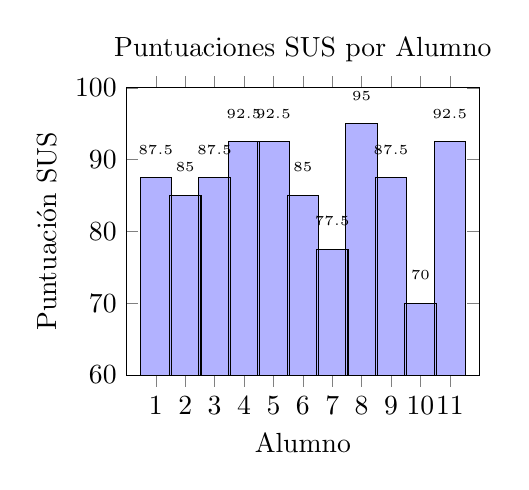
\begin{tikzpicture}
		\begin{axis}[
			ybar,
			title={Puntuaciones SUS por Alumno},
			xlabel={Alumno},
			ylabel={Puntuación SUS},
			ymin=60,
			ymax=100,
			xtick=data,
			xticklabels={1,2,3,4,5,6,7,8,9,10,11},
			width=0.5\textwidth,
			bar width=0.4cm,
			nodes near coords,
			nodes near coords align={vertical},
			every node near coord/.append style={font=\tiny, yshift=5pt}
			]
			\addplot[fill=blue!30] coordinates {
				(1,87.5) (2,85.0) (3,87.5) (4,92.5) (5,92.5)
				(6,85.0) (7,77.5) (8,95.0) (9,87.5) (10,70.0) (11,92.5)
			};
		\end{axis}
	\end{tikzpicture}
	\caption{Distribución individual de usabilidad percibida.}
	\label{fig:barras}
\end{figure}
\begin{figure}[H]
	\centering
	\begin{tikzpicture}
		\pie[
		text=legend,
		explode={0.1,0,0},
		color={green!30,blue!30,red!30},
		sum=auto,
		before number=\sffamily,
		after number=\sffamily\%
		]{
			72.7/\textbf{Excelentes} ($\geq$85),
			27.3/\textbf{Aceptables} (68-84),
			0/\textbf{Inaceptables} ($<$68)
		}
	\end{tikzpicture}
	\caption{Distribución de usabilidad según SUS (11 alumnos). \\ 
		\textbf{Excelentes}: 8 alumnos (72.7\%), \textbf{Aceptables}: 3 alumnos (27.3\%), \textbf{Inaceptables}: 0 alumnos (0\%).}
	\label{fig:sus_pie}
\end{figure}



\subsubsection{Análisis del Net Promoter Score (NPS)}

El Net Promoter Score (NPS) me pareció especialmente revelador porque no solo mide satisfacción, sino lealtad real. Al preguntar a mis compañeros \textit{"¿Qué probabilidad hay de que recomiendes este teclado VR?"}, sus respuestas (Tabla \ref{tab:nps_scores}) mostraron un patrón curioso. Casi todos dieron puntuaciones altas - entre 7 y 9 - pero con matices que los números solos no capturan completamente.

Fíjate en el gráfico de barras (Figura \ref{fig:nps_symbolic}): ese vacío entre 0 y 6 salta a la vista. ¡Ni un solo detractor! Eso ya es alentador. Pero lo interesante fue cómo se agruparon las respuestas: cinco compañeros pusieron 8 (neutros), cuatro dieron 9 (promotores), y solo dos se quedaron en 7. Esto me hizo preguntarme: ¿por qué nadie dio el 10 máximo? En charlas posteriores, varios mencionaron que "para recomendar algo a un cliente" querrían probar antes la versión definitiva.

Con esos números, el cálculo del NPS quedó en 45.5 (Figura \ref{fig:nps_torta}). Según los estándares tecnológicos, se considera una puntuación positiva - claramente por encima de lo mediocre - aunque personalmente esperaba algo más alto. Al desmenuzarlo, entendí mejor: tenemos un 45.5\% de promotores entusiastas, pero más de la mitad (54.5\%) se mantuvo neutral. Es como si dijeran \textit{"Funciona, pero no lo recomendaría sin reservas"}.

Al cruzar esto con los resultados SUS, encontré coherencia. Quienes dieron mejores puntuaciones de usabilidad (como ese SUS de 95 del Alumno 8) fueron justo los que pusieron 9 en NPS. El caso del Alumno 10 resultó ilustrativo: 70 en SUS y 7 en NPS - en ambos casos el más bajo. Cuando hablamos después, me dijo: \textit{"La idea mola, pero para proyectos serios echo en falta más personalización"}.

La verdad es que aunque matemáticamente 45.5 es "bueno", lo valioso está en los detalles: esos cuatro que dieron 9 serían nuestros primeros evangelizadores. Y los cinco de puntuación 8... bueno, ahí está nuestro reto principal. Con ajustes específicos, podríamos convertirlos en promotores.

\begin{table}[h]
	\centering
	\caption{Puntuaciones NPS por Alumno}
	\label{tab:nps_scores}
	\begin{tabular}{|c|c|}
		\hline
		\textbf{Alumno} & \textbf{Puntuación (0-10)} \\ \hline
		1 & 8 \\ \hline
		2 & 8 \\ \hline
		3 & 7 \\ \hline
		4 & 9 \\ \hline
		5 & 9 \\ \hline
		6 & 8 \\ \hline
		7 & 8 \\ \hline
		8 & 9 \\ \hline
		9 & 9 \\ \hline
		10 & 7 \\ \hline
		11 & 8 \\ \hline
	\end{tabular}
\end{table}

% Gráficos existentes (se mantienen igual)
\begin{figure}[h]
	\centering
	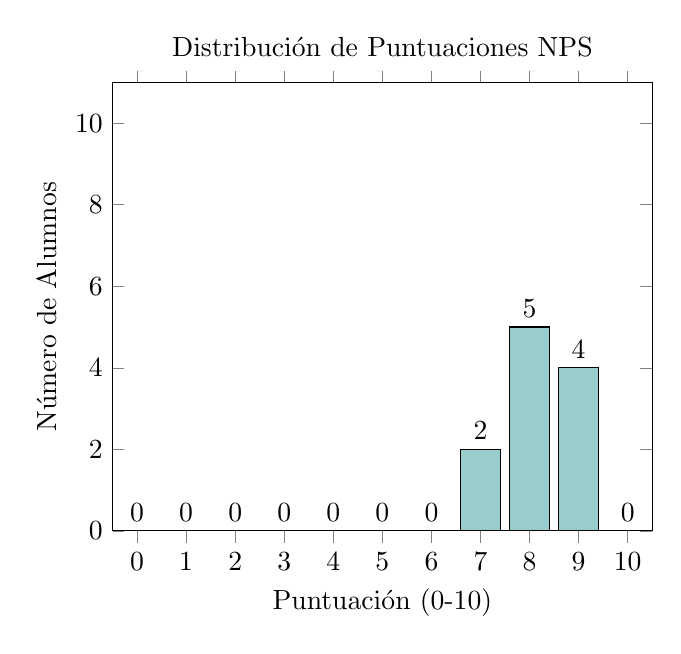
\begin{tikzpicture}
		\begin{axis}[
			ybar,
			title={Distribución de Puntuaciones NPS},
			xlabel={Puntuación (0-10)},
			ylabel={Número de Alumnos},
			ymin=0,
			ymax=11,
			xtick=data,
			symbolic x coords={0,1,2,3,4,5,6,7,8,9,10},
			bar width=0.5cm,
			nodes near coords,
			enlarge x limits=0.05,
			]
			\addplot[fill=teal!40] coordinates {
				(0,0) (1,0) (2,0) (3,0) (4,0) (5,0) (6,0)
				(7,2) (8,5) (9,4) (10,0)
			};
		\end{axis}
	\end{tikzpicture}
	\caption{Distribución completa de respuestas NPS. Destaca la ausencia de puntuaciones bajas (0-6) y la concentración en 7-9.}
	\label{fig:nps_symbolic}
\end{figure}

\begin{figure}[h]
	\centering
	\begin{tikzpicture}
		\pie[
		text=legend,
		explode={0.1,0,0},
		color={green!30,blue!30,red!30},
		sum=auto
		]{45.5/Promotores, 54.5/Neutros, 0/Detractores}
	\end{tikzpicture}
	\caption{Proporción NPS: casi mitad y mitad entre promotores y neutros. Los detractores brillan por su ausencia.}
	\label{fig:nps_torta}
\end{figure}

\subsection{Video de demostración}

Se adjunta un video demostrativo con el funcionamiento del sistema:  
\url{https://youtu.be/DTkw49Uq6r4}.